
\documentclass[12pt]{article}

\usepackage[T1]{fontenc}
\usepackage{float}
\usepackage[utf8]{inputenc}
\usepackage[french]{babel}
\usepackage{amsmath}
\usepackage{amssymb}
\usepackage[top=1.5cm, bottom=1.5cm, left=1.5cm, right=1.5cm]{geometry}
\usepackage{graphicx}
\usepackage{multicol}
\usepackage{lipsum}
\usepackage{eurosym}
\usepackage{indentfirst}
\usepackage{titlesec}
\usepackage{pifont}
\usepackage{url}
\usepackage{epsf}
\usepackage{listings}
\newcommand\tab[1][1cm]{\hspace*{#1}}
\begin{document}
    \begin{titlepage}
        \newcommand{\HRule}{\rule{\linewidth}{0.5mm}}
        \center
        \textsc{\LARGE
        UNIVERSITE CAEN-NORMANDIE
        } \\[1cm]
        
\includegraphics[scale=1]{images/LOGO-UNICAEN_V-2.2-N} \\[1cm]
        \HRule \\[0.4cm]
        { \huge \bfseries Rapport de développement: EASYTASK\\[0.15cm] }
        \HRule \\[1.5cm]
        KITSOUKOU Manne Emile\\[1cm]
        ALSEINY
        \\[1cm]
        \textbf{Licence 3 Informatique}\\
        \today \\ [1cm]
    \end{titlepage}
    \newpage
    \tableofcontents
    \newpage
    \section{Introduction}{\label{sec:intro}}

        Dans le cadre de la validation de l'UE( Unité d'Enseignement) de \textbf{Développement d'application web client},
        nous avons été amenés à réaliser une application de gestions de tâches. L'objectif de ce projet était de mettre
        en place une interface utilisateur intuitive, fonctionnel et ergonomique permettant à un utilisateur de gérer
        ses listes de tâches de maniere simple et efficace.\\

        Ce projet nous a permis de découvrir le framework \textbf{React native } tout en mettant en pratique nos
        connaissances en développement d'application mobiles. Nous avons dû faire face à des défis liés à la prise
        en main de ce nouvel outil, mais avons réussi à mettre en place une application fonctionnelle et ergonomique
        respectant les exigences de l'énoncé du projet. Cela a été également l'occassion de mettre en pratique nos
        connaissances des bases de données non traditionnelles à travers la mise en place d'une base de données
        \textbf{NoSQL} \textbf{GRAPHQL} à travers le service \textbf{Apollo NEO4J}.

        \section{Présentation de l'application}{\label{sec:app}}
        EASYTASK est une application de gestion de tâches. Elle permet à un utilisateur de créer des listes de tâches
        et de les gérer. Le développement à travers le framework \textbf{React native} permet de pouvoir utiliser
        l'application sur la plateformes \textbf{Android}, \textbf{IOS} et \textbf{Web}. Cela permet de rendre l'application
        plus accessible au plus grand nombre d'utilisateurs.\\
        L'application est divisée en différents écrans. Cette séparation permet de rendre l'application plus
        ergonomique et intuitive. L'utilisateur peut naviguer entre les différents écrans à travers des boutons
        présents sur chaque écran.\\

        \subsection{Ecrans d'authentification}{\label{subsec:auth}}
        L'application nécessite une authentification pour pouvoir accéder aux fonctionnalités de l'application.
        L'utilisateur doit donc se connecter à l'application à travers un formulaire d'authentification.\\
        \begin{figure}[H]
            \centering
            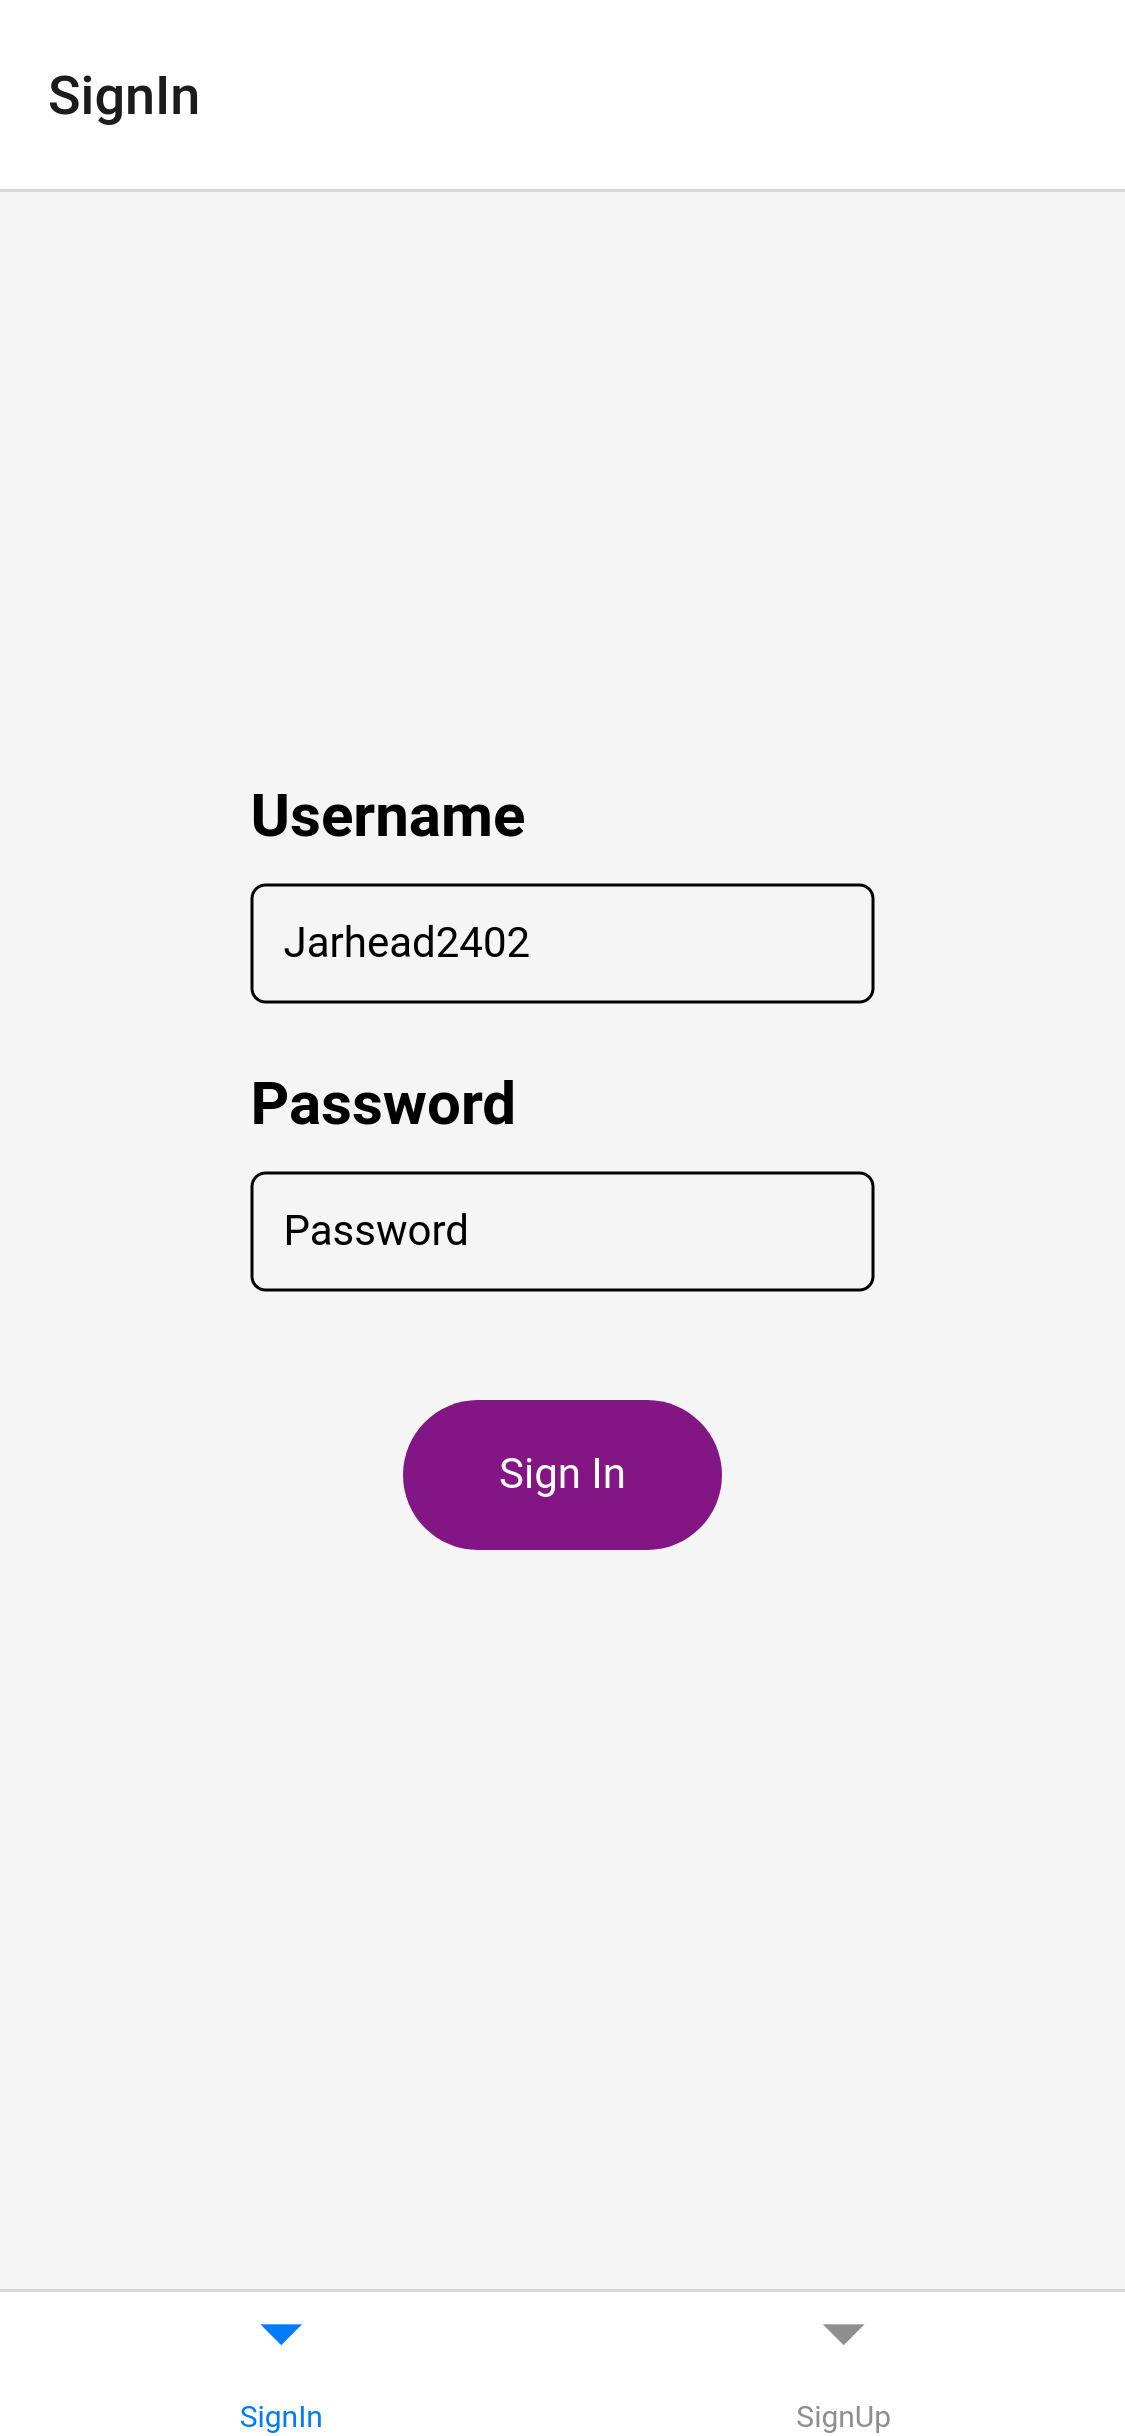
\includegraphics[width=0.4\textwidth]{images/signIn}
            \caption{Ecran d'authentification}
            \label{fig:auth}
        \end{figure}
        L'utilisateur doit renseigner son nom d'utilisateur et son mot de passe pour pouvoir accéder à l'application.
        Si l'utilisateur n'a pas de compte, il peut s'inscrire en cliquant sur le bouton \textbf{S'inscrire} présent
        en bas de l'écran.\\
        \begin{figure}[H]
            \centering
            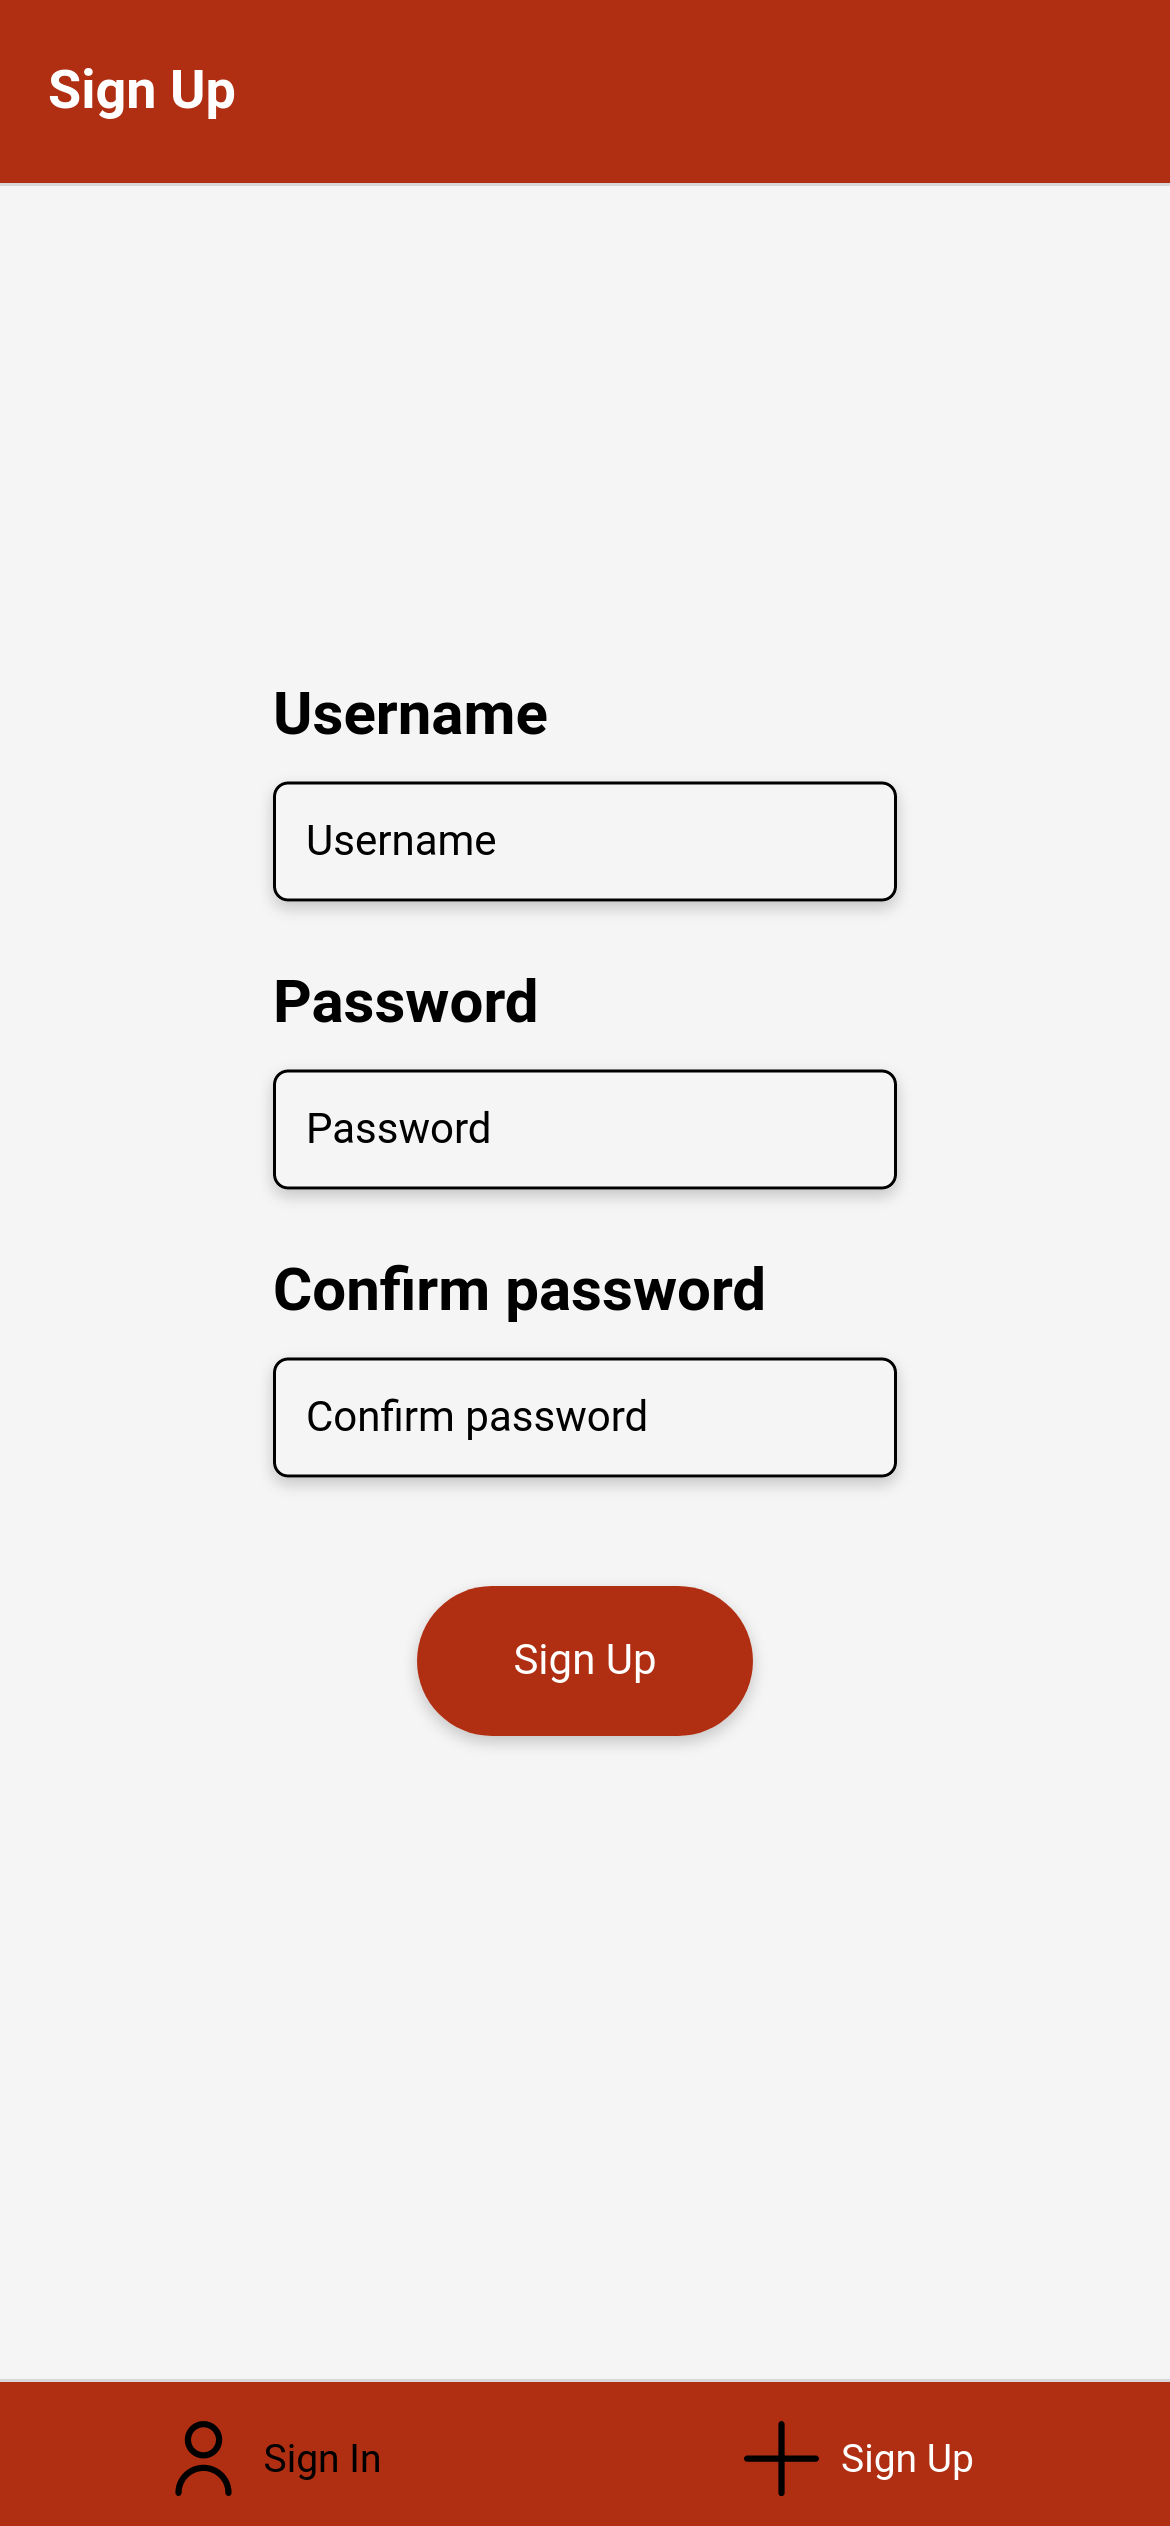
\includegraphics[width=0.4\textwidth]{images/signUp}
            \caption{Ecran d'inscription}
            \label{fig:insc}
        \end{figure}
        L'utilisateur doit renseigner son nom d'utilisateur, son mot de passe et sa confirmation.\\

        Cependant il faut noter que la réalisation de l'authentification reste basique.

        \subsection{Ecrans de gestion des listes de tâches}{\label{subsec:task}}
        Nous utilisons 2 ecrans pour gérer les listes de tâches. En effet, nous donnons la possibilités à l'utilisateurs
        de pouvoir manipuler plusieurs listes de taches. De ce fait, nous devrions avoir un écran principales qui permet
        d'afficher l'ensemble des listes de taches.
        \begin{figure}[H]
            \centering
            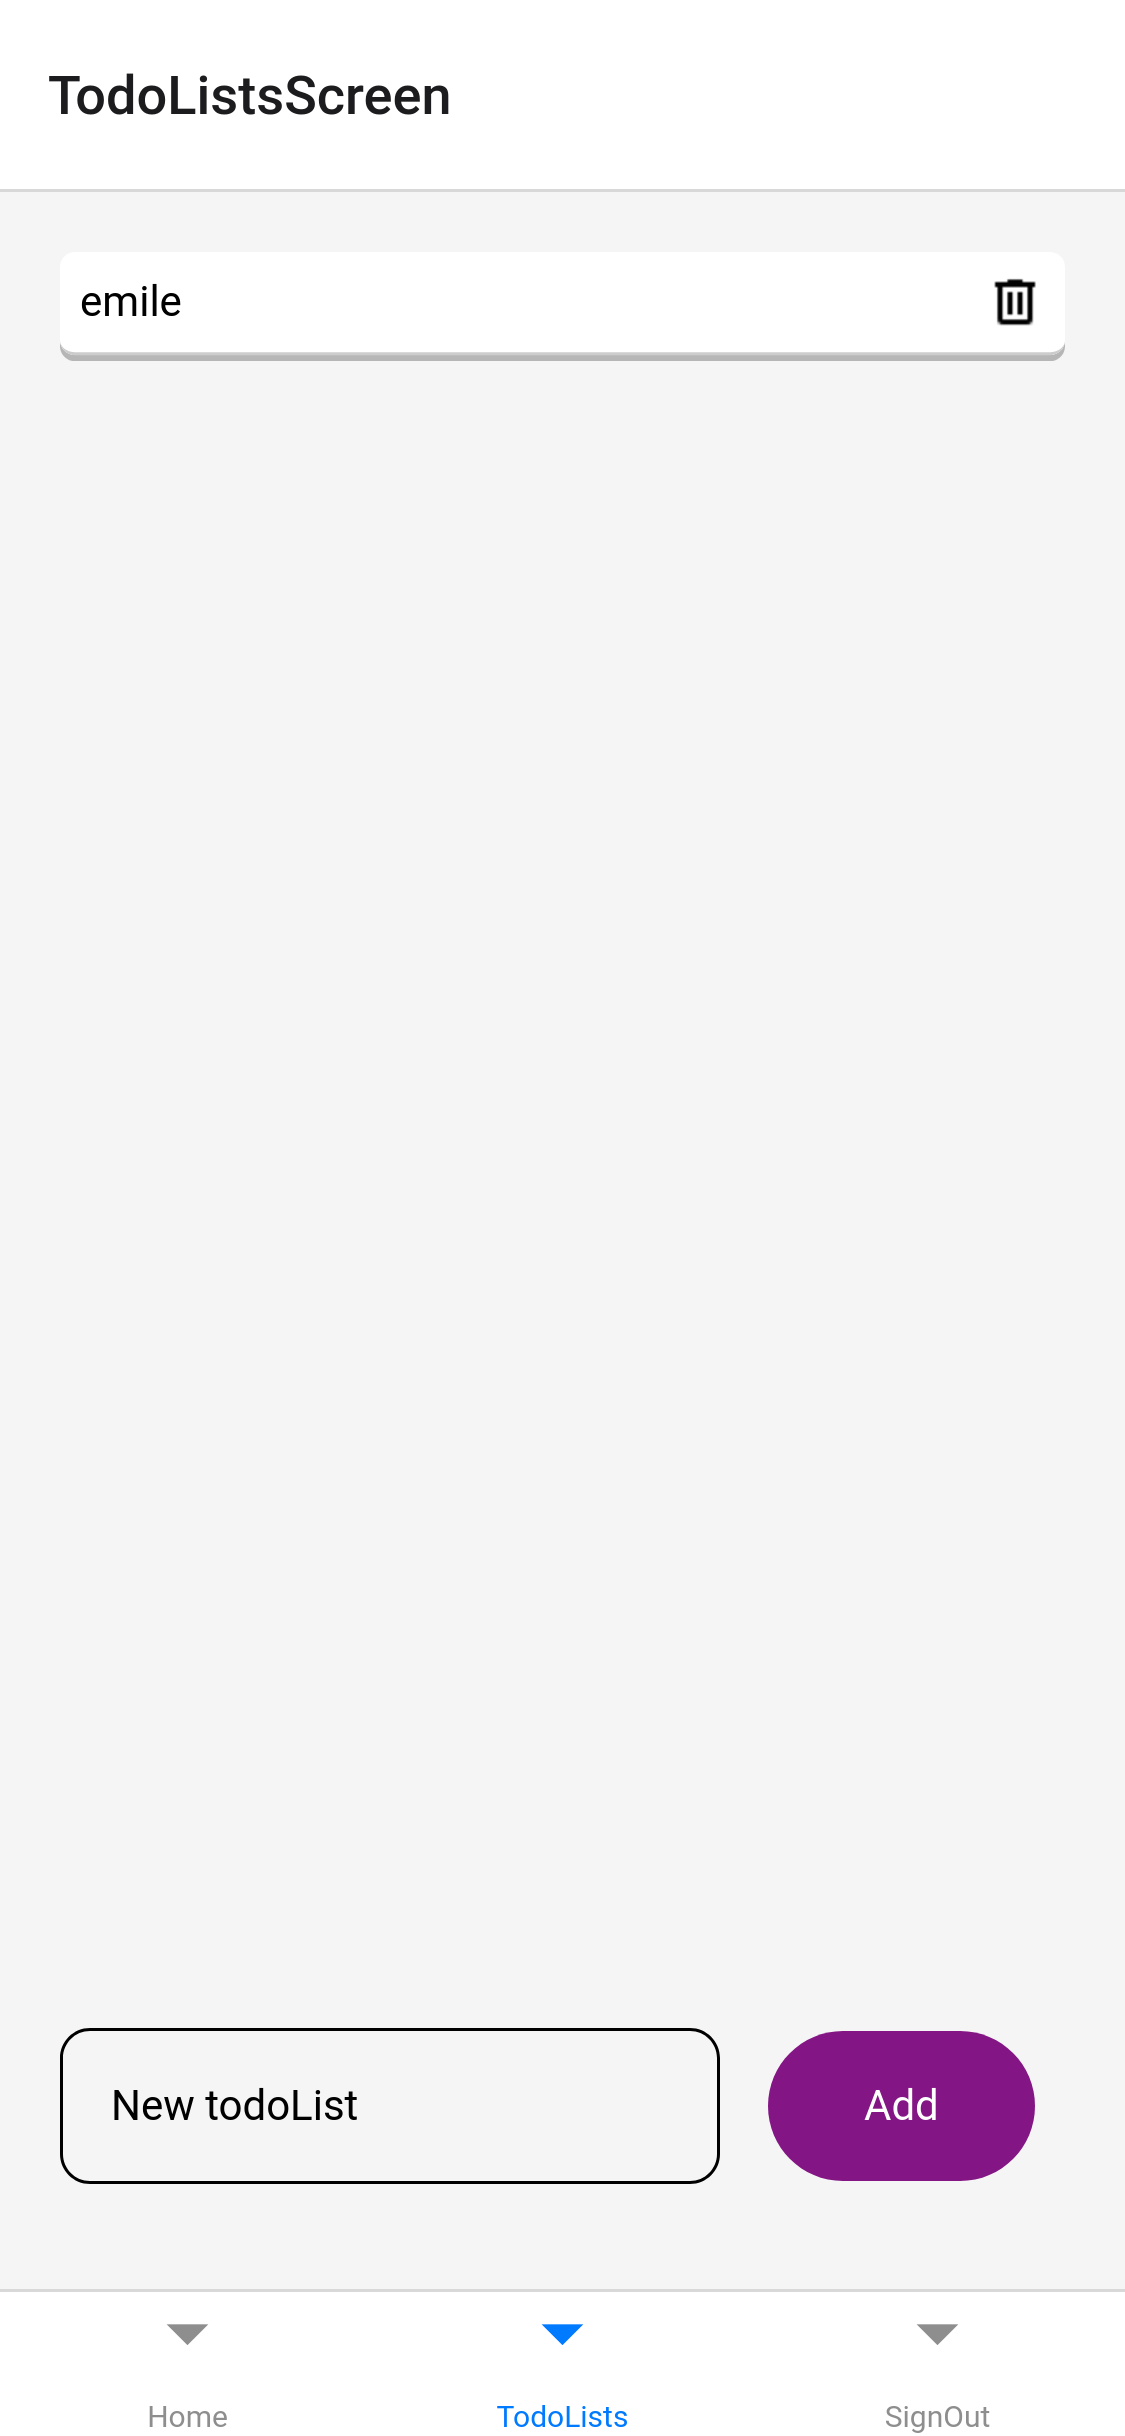
\includegraphics[width=0.2\textwidth]{images/taskList}
            \caption{Ecran de gestion des listes de tâches}
            \label{fig:taskList}
        \end{figure}
        L'utilisateur peut créer une nouvelle liste de tâches en cliquant sur le bouton \textbf{Nouvelle liste} présent
        après avoir renseigné le nom de la liste. Il peut également supprimer une liste de tâches en cliquant sur la poubelle
        présente à droite de chaque liste.\\
        En cliquant sur une liste de tâches, l'utilisateur est redirigé vers un écran qui lui permet de gérer les tâches
        de la liste.\\
        \begin{figure}[H]
            \centering
            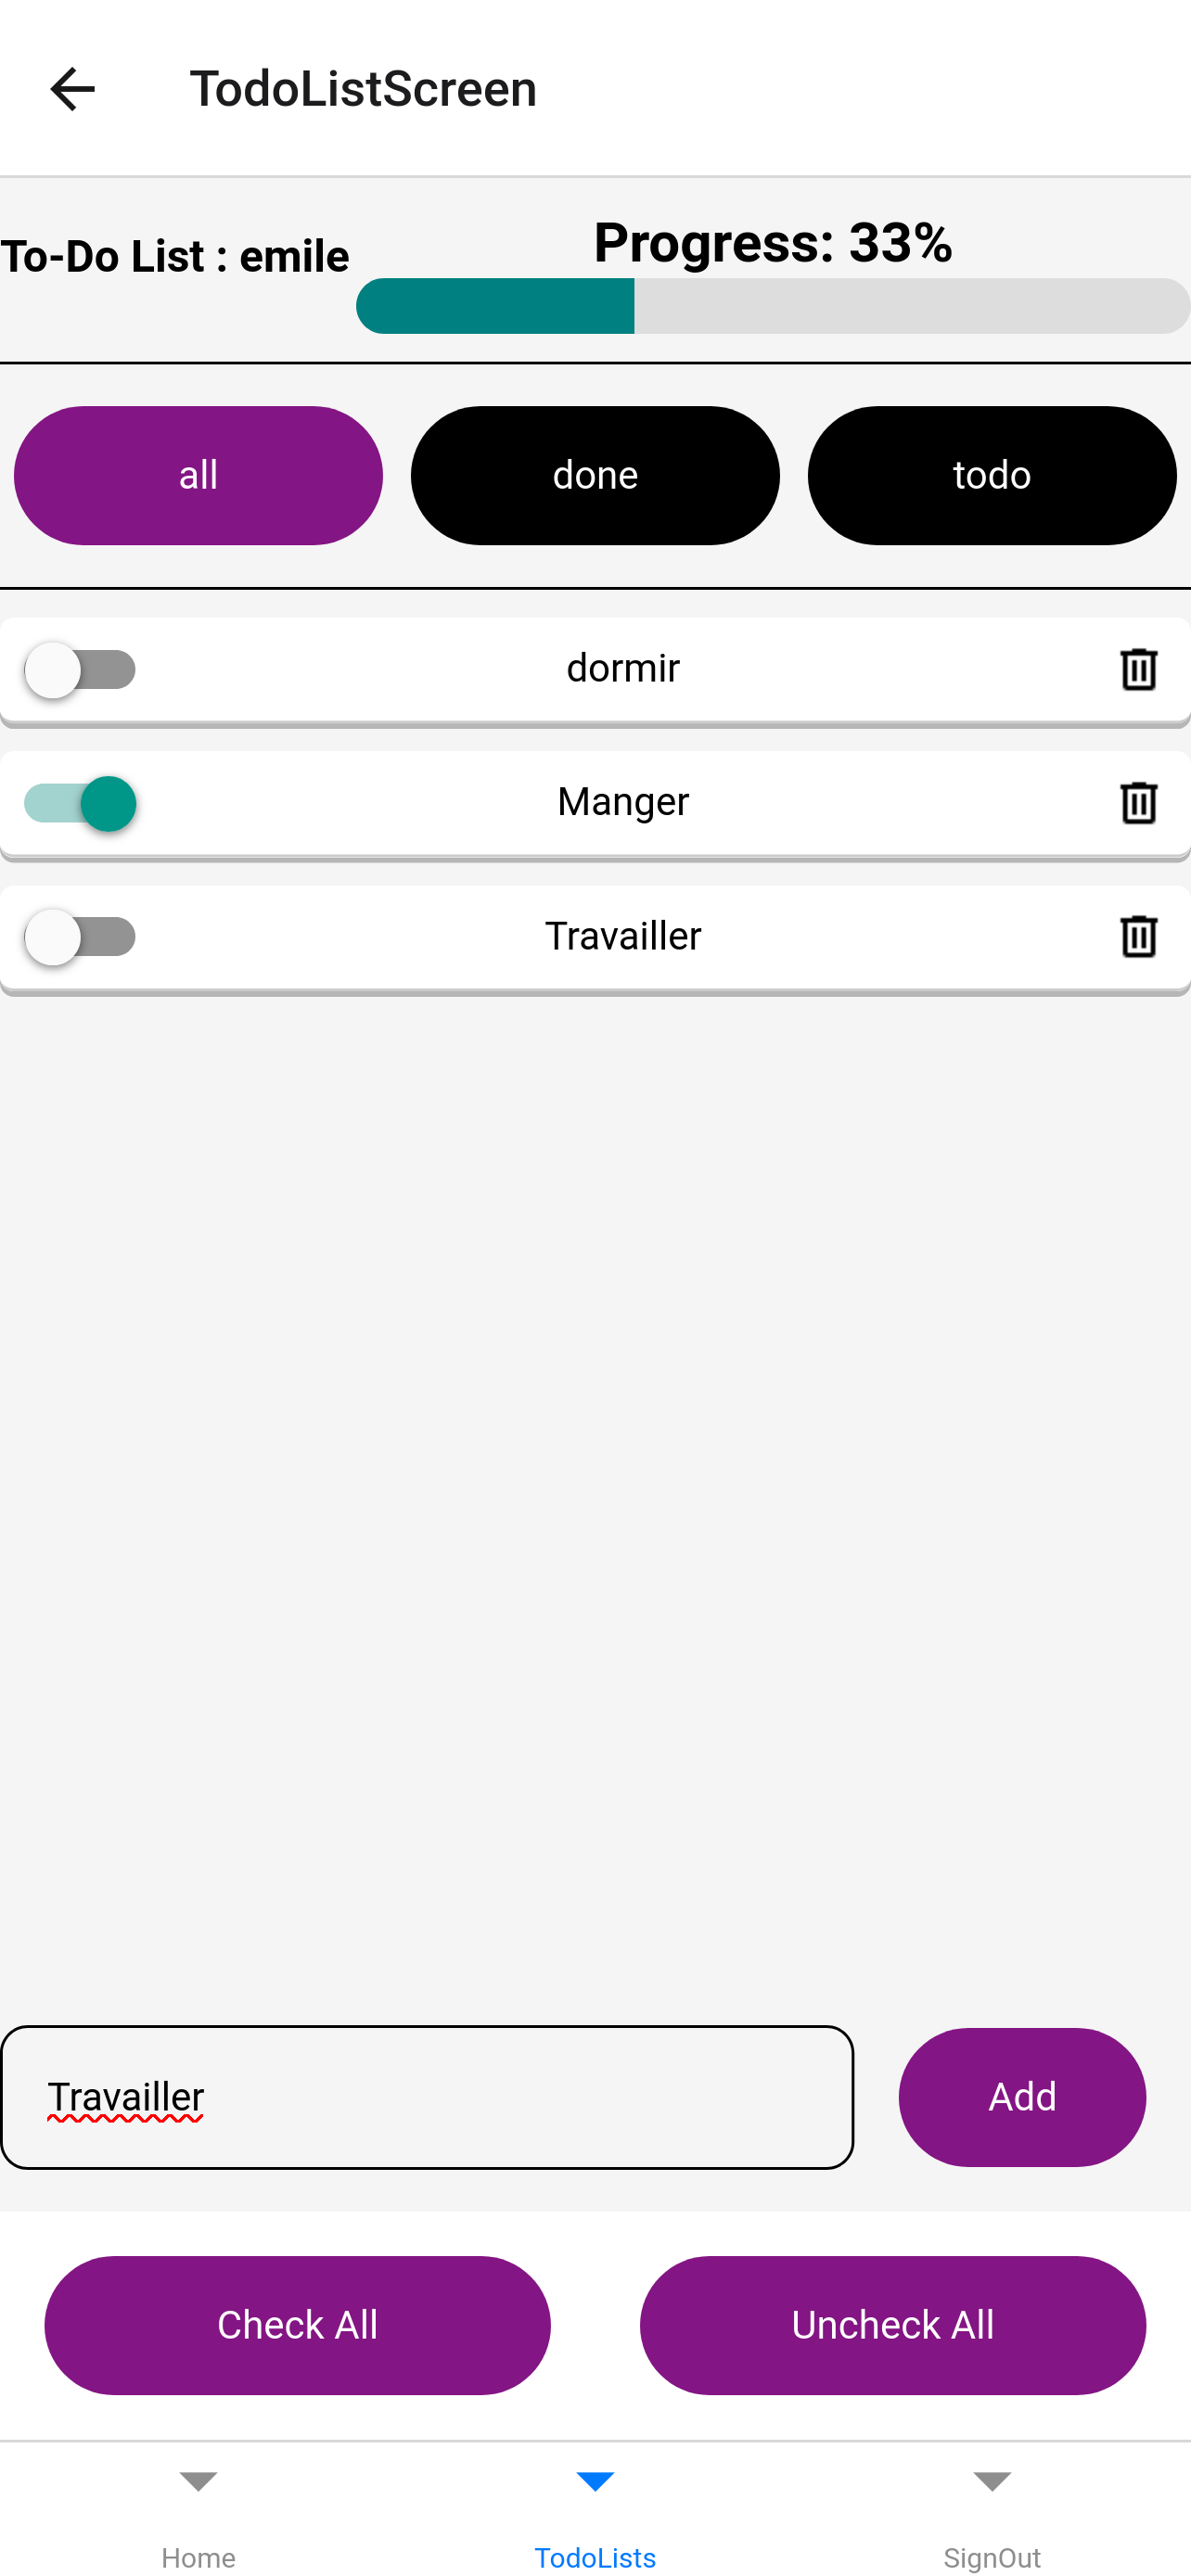
\includegraphics[width=0.4\textwidth]{images/tasks}
            \caption{Ecran de gestion des tâches}
            \label{fig:task}
        \end{figure}
        L'utilisateur peut créer une nouvelle tâche en cliquant sur le bouton \textbf{Nouvelle tâche} présent
        après avoir renseigné le nom de la tâche. Il peut également supprimer une tâche en cliquant sur la poubelle.
        Par défaut à la creation d'une tâche, elle est considérée comme non terminée. L'utilisateur peut la terminer
        en cliquant en sur le switch présent à droite de la tâche. Dans ce cas, la tâche est considérée comme terminée
        et est désormais grisé.\\
        Différents filtres sont disponibles pour afficher les tâches. L'utilisateur peut afficher;
        \begin{itemize}
            \item Les tâches non terminées
            \item Les tâches terminées
            \item Toutes les tâches
        \end{itemize}
        Il a aussi la possibilité de rendre toutes les tâches terminées (resp non terminées) en cliquant sur le bouton
        \textbf{Tout terminer} (resp \textbf{Tout non terminer}).

        \subsection{Autres écrans}{\label{subsec:other}}
        Nous avons aussi développé d'autres écrans comme l'écran de déconnexion, l'écran d'accueil.
        Ces écrans sont intermédiaires entre les écrans de gestion des listes de tâches et les écrans d'authentification.
            % Ajout des images des autres écrans

        \section{Développement de l'application}{\label{sec:dev}}
        Nous avons développé l'application à travers le framework \textbf{React native}. Ce framework permet de développer
        des applications mobiles multiplateformes. Il permet de développer des applications pour les plateformes
        \textbf{Android}, \textbf{IOS} et \textbf{Web}.\\
        Outre les composants natifs de React native, nous avons implémenté d'autres composants réutilisables. En effet,
        l'intérêt de React native est de pouvoir réutiliser des composants. Cela permet de rendre le code plus lisible
        et plus maintenable.\\

    \subsection{Composants réutilisables}{\label{subsec:comp}}

    \subsubsection{Field}{\label{subsubsec:field}}
    Ce composant permet de créer un champ de formulaire. Il prend en paramètre le type du champ, le nom du champ,
    la valeur du champ, la fonction de mise à jour de la valeur du champ et un booléen qui indique si le champ est
    obligatoire ou non.\\
    Il a été implémenté, car nous avons eu besoin de créer plusieurs champs de formulaire. Ainsi pour éviter de
    répéter le code et/ou du style, nous avons créé un composant réutilisable. Cela a permit d'avoir une uniformité
    dans l'application à tout endroit où nous avons utilisé ce composant.\\

    \subsubsection{ButtonComponent}{\label{subsubsec:button}}
    Les buttons sont l'un des composants les plus utilisés dans une application. Il peut sembler etrange et inutile
    de créer un composant réutilisable pour un bouton étant donné que React native propose déjà un composant. Cependant,
    nous avons eu besoin de créer un bouton avec un style particulier. En effet, le composant natif de React native
    ne laisse pas une grande liberté sur le style du bouton.\\
    Ce composant réutilisable a permis de créer des boutons à une allure unique et uniforme dans l'application. Il est
    assez distinct des boutons natifs de React native et apporte une touche d'originalité à l'application.\\

    \subsubsection{IconComponent}{\label{subsubsec:icon}}
    Nativement, React native ne propose pas de composant pour afficher des icones. Cependant, il existe des librairies
    qui permettent d'afficher des icones. Cependant, l'utilisation de ces librairies n'est pas très pratique et
    implique non seulement l'installation de libraries supplémentaires mais aussi une dépendance à ces libraries.\\
    Nous avons donc créé un composant réutilisable qui permet d'afficher des icones. Son utilisations est très simple
    et assez similaire à ceux proposés par les librairies.\\

    \subsubsection{Item}{\label{subsubsec:item}}
    Il a été remarqué durant le developpement que nous avions besoin de créer des items pour afficher des informations
    dans différentes listes. Par exemple, nous avons besoin d'afficher des listes de tâches dans une liste. Nous avons
    ainsi créé un composant réutilisable qui permet de créer des items.\\
    Le composant créé peut être cliquable, switchable, et/ou supprimable. Ces divers propriétés n'influencent pas
    (ou grandement pas) le style/la manière d'affichage de l'item.\\

    \subsubsection{ListItems}{\label{subsec:list}}
    Une liste d'item peut être nativement représentée par un composant \textbf{FlatList} de React native. Cependant,
    pour avoir une meilleure expérience utilisateur, nous avons décidé d'utiliser un composant personnalisé qui nous a
    permis de décorer la liste d'item à partir d'une \textbf{FlatList}.\\
    Toutefois sa création n'est qu'une simple surcouche de la \textbf{FlatList} de React native. Et donc, nous pouvons
    facilement basculer vers l'utilisation de la \textbf{FlatList} si nous le souhaitons.\\

    \subsection{Architecture}{\label{subsec:arch}}
    L'architecture d'un projet en \textbf{React native} n'est pas si différente de celle d'un projet web. Toutefois
    il existe quelques différences essentielles.
    \subsubsection{Structure des fichiers}{\label{subsubsec:structure}}
    La structure des fichiers d'un projet en \textbf{React native} est la suivante :
    \begin{itemize}
        \item \textbf{android} : contient les fichiers spécifiques à l'application pour la plateforme Android.
        \item \textbf{ios} : contient les fichiers spécifiques à l'application pour la plateforme IOS.
        \item \textbf{node_modules} : contient les modules nodejs utilisés par l'application.
        \item \textbf{src} : contient les sources de l'application.
        \item \textbf{assets} : contient les ressources statiques de l'application.
        \item \textbf{components} : contient les composants réutilisables de l'application.
        \item \textbf{screens} : contient les écrans de l'application.
        \item \textbf{services} : contient les services de l'application.
        \item \textbf{App.js} : fichier principal de l'application.
        \item \textbf{app.json} : fichier de configuration de l'application.
        \item \textbf{package.json} : fichier de configuration du projet.
    \end{itemize}

    \subsection{Navigation}{\label{subsec:navigation}}
    La navigation dans une application \textbf{React native} est gérée par un composant natif appelé \textbf{NavigationContainer}.
    Ce composant permet de gérer la navigation dans l'application.\\
    Il existe plusieurs types de navigation dans une application \textbf{React native}. Nous avons choisi d'utiliser
    la navigation par \textbf{BottomTabNavigator} qui permet de naviguer entre plusieurs écrans en utilisant des
    onglets en bas de l'écran.\\
    La navigation par \textbf{BottomTabNavigator} est gérée par un composant natif appelé \textbf{createBottomTabNavigator}.
    Ce composant permet de créer un \textbf{BottomTabNavigator} à partir d'une liste d'écrans.\\

    \subsection{Services}\label{subsec:services}
    Les services sont des classes qui permettent de diriger les communications avec les serveurs.\\
    Nous avons utilisé la librairie \textbf{axios} pour gérer les communications avec les serveurs.\\
    Nous avons créé un service par type de communication avec le serveur.\\
    La liste des services est la suivante :
    \begin{itemize}
        \item \textbf{Auth} : gère les communications avec le serveur pour l'authentification.
        \item \textbf{Task} : gère les communications avec le serveur pour les tâches.
        \item \textbf{User} : gère les communications avec le serveur pour les utilisateurs.
        \item \textbf{TaskList} : gère les communications avec le serveur pour les listes de tâches.
    \end{itemize}

    \subsection{Context}\label{subsec:context}
    Les contextes sont des objets qui permettent de partager des informations entre les composants de l'application.
    Nous avons utilisé la librairie \textbf{react-native-context-api} pour gérer les contextes.\\
    Nous avons créé un contexte par type d'information à partager.\\
    La liste des contextes est la suivante :
    \begin{itemize}
        \item \textbf{Auth} : gère les informations de l'utilisateur connecté.
        \item \textbf{Task} : gère les informations des tâches.
        \item \textbf{TaskList} : gère les informations des listes de tâches.
        \item \textbf{User} : gère les informations des utilisateurs.
    \end{itemize}


\end{document}